\documentclass[main.tex]{subfiles}
\begin{document}


\chapter{Fazit}

Aus den erstellten Prototypen und der Evaluation sind viele Erkenntnisse zusammengekommen die hier noch Zusammengefasst werden. 

\section{Implementation}

\subsubsection{JasperReports}
Kleinere Problemen bei der Umsetzung haben die Entwicklung etwas gehindert wie die  Probleme mit Bold. Das iReport zeigte es richtig an aber es wurde nicht in die PDFs übernommen. Dennoch war iReport sehr gut, einfache Handhabung und gute Unterstützung für die Erstellung der Templates. Generierte Reports sind auch als Kompilierte  jasper-Files noch verständlich.  


\subsubsection{Apache PdfBox}
Zeilenumbruch in für einen langen Text muss selber entwickelt werden. Gleiches gilt für die Seitenumbrüche für lange Texte ist eher umständlich. Es fehlt ein High-Level API darum ist es eher schwierig Templates zu erstellen, da diese immer auf der Basis von spezifischer Daten-Inputs basieren und eine dynamische Ansicht mit einem Flow-Pattern ist eher schwierig. Ausrichten von Textblöcke wird anhand der Seitengrösse  programmiert somit ist auch im Textmodus schwierig eine Tabelle zu kreieren mit mehrzeiligen Zelleninhalten.

Dennoch bietet sich Apache PDF an pixelgenaue Layouts zu erstellen, da die Texte mit Offset-Angaben ausgerichtet werden können. 

\subsubsection{iText}
Es fühlt sich an als schreibe man eine Worddokument, die \acrlong{api} ist einfach und klar, Seiten werden automatisch neu generiert. Es benötigt keine Seitenangaben wie Rand und Grösse da Standards diese bereits vorgeben. Ein Standard-Set an Fonts wird als Konstanten mitgegeben. Hersteller bietet viele Beispiele und Hilfreiche Blogs an. 
Positionierung einzelner Elemente kann über die Canvas Funktionen ebenfalls erreicht werden z.B.  bei definieren von Footer oder Header. 
iText lässt auch zu dokumentübergreifende Fonteinstellung zu definieren was die Entwicklung erleichtert. 
Doch auch hier ergeben sich Probleme mit den Fussnoten, das Dokument müsste erneut bearbeitet werden um die Anzahl Seiten zu kennen da diese beim erstellen noch nicht bekannt sind. Beim erstellen einer neuen Seite ist die vorhergehende immer um eins kleiner da beim erstellen der Seite nicht bekannt war das eine weitere Seite zu erstellen ist.


\section{Performance}



\subsection{Throughput}
% Welcher der Services hat am Meisten Durchsatz an den Tag gelegt ? 

Der höchste Durchsatz wurde mit ApachePDFBox erreicht, gefolgt von iText und dann JasperReports. Die Analyse des Durchsatzes nach Bytes hat jedoch ergeben das dieser fast konstant blieb. Allenfalls ist dies ein Hinweis auf ein Engpass in der Netzwerkbandbreite. 

\subsection{Latency}
Auch bei der Latency by Request ist Apache PDFBox am schnellsten, die Verarbeitung kann bei den ersten zwei Szenarien unterhalb einer Sekunde durchgeführt werden was bei JasperReports nicht der Fall ist. iText wiederum hat nur leicht längere Latenzzeiten. 

\subsection{Verfügbarkeit}

Keine der Test ist jemals ausgefallen, es haben sich auch keine Fehler ereignet die von JMeter als solche identifiziert wurden.
Die meisten Test haben sich über die Zeitspanne von 10 Stunden erstreckt, dabei haben  die Logs ebenfalls keine Ausfälle nachgewiesen. 

Dennoch hat JasperReports sehr lange Antwortszeiten die ebenfalls zu TimeOuts füren könnten somit also die Verfügbarkeit beeinschränkt.

\section{Ressources}

\subsection{RAM}
Der Verbrauch von RSS-Memory ist sowohl bei iText und Apache PDFBox meisst unterhalb der Memory-Quoata. Der SWAP wird einzig von JasperReport genutzt und erklärt auch wohl die lange Verarbetitungszeit. Sowie wird der SWAP nicht wieder freigegeben was zu einer Memory-Blase führt. 



\subsection{CPU}
Die CPU Last hat nur bei JasperReports einen durgänginge Spitzen angezeigt, Apache PDFBox hat hier wiedermal Ressourcenschonend gearbeitet. iText hat einen nichterklärbaren tiefe CPU Last im Szenario 3.  


\section{Wer ist nun der Performanteste?}

\begin{figure}[!hb]
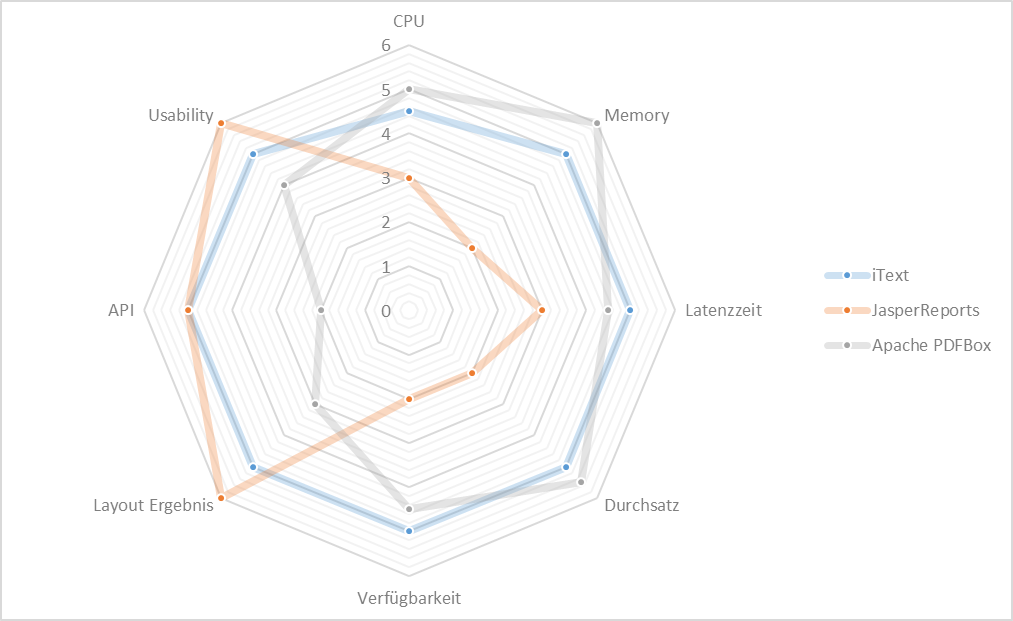
\includegraphics[width=\textwidth]{end/5_erfarhungsbericht/Netzdiagramm.png}
 \caption{Netzdiagramm nach Metrik}
 \label{figure:netzdiagrammMetriken}
\end{figure}

Würde man für diese Frage einzig und alleine die Daten des Durchsatzes nehmen müsste man sagen es ist im Durchschnitt Apache PDFBox. Trotz des Szenario 3 erreicht dieser \acrlong{osre} immer noch durchschnittlich 70 Anfragen pro Sekunde. Gefolgt von iText mit 30 Anfragen pro Sekunde und dann JasperReports mit 14.5 Anfragen pro Sekunde im Durchschnitt. 

Das 95\% Perzentil sagt wiederum das JasperReports das schnellste \acrlong{osre} ist und das nur weil das Szenario 3 die Antwortszeiten in die Höhe getrieben haben.

Pauschal lässt sich sagen das mit Apache PDFBox die höchste Performanz, Ressourcennutzung und Antwortszeiten erreichen lässt. Dennoch haben auch die anderen \acrlong{osre}s gute Seiten die in verschiedenen Anwendungsfälle besser einzusetzen sind. In der Abbildung \ref{figure:netzdiagrammMetriken} lassen sich die Tendenzen der jeweiligen \acrlong{osre} erkennen. 

\subsection{Apache PDFBox}
Hat klare stärken was die technische Performance angeht. 
Die Umsetzung ist klar auch historisch geprägt, es ist ein Tool primär zu Extraktion von Daten und nicht für die Erstellung von Reports gedacht. Was es auch so performant macht. Das geeignete Einsatzgebiet im Umfeld von Reportserstellung sind im Zusammenhang von statischen Layouts wie Flugtickets oder Konzertkarten. 


\subsection{iText}
iText wurde kreiert genau um Reports zu generieren, dies ist klar erkennbar an dem versatillen und umfangreichen \acrlong{api}. Es beherrscht auch komplexere PDF-Aufbau ohne Performaceverlust. Für einen Online-Einsatz als brauchbar empfunden. Da das API gut genug ist um Reports leicht verständlich zu Codieren und darum wartbar bleiben.

\subsection{JasperReports}
Es hat klare Vorteile Reports visuell aufzubereiten, leider hat aber diesen Vorteil keine nutzbare Performance für eine Online-Verarbeitung gezeigt. Was bedeutet JasperReports in einem Microservice einzusetzen ist nur sehr bedingt geeignet. Geeignetes Einsatzgebiet wären klar zeitlich definierte Reportgenerierungen. Oder auch wenn komplexe Reports womöglich  von Nicht-Entwickler definiert werden sollen, dafür ist iReport ein geeignetes Hilfsmittel.  

\section{Ausblick}

Aus den Peformancemessungen entstanden einige Fragen im Zusammenhang mit der Implementation die noch zu adressieren sind wie z.B.: 
\begin{itemize}  
    \item Sind Engpässe in der Applikation oder Netzwerk Ursachen für die schlechte Performance? 
    \item Sind Fehler in der Applikation die unnötigen Programmcode ausführen?
    \item Sind Einstellungen möglich um Zugriffe auf Dateien wie Bilder zu verbessern?
\end{itemize}
Und in dieser Arbeit nicht addressierbaren Fragen bezüglich Skalierbarkeit der PaaS.
\begin{itemize}  
    \item Mit welcher Anzahl Server können X Anzahl User performant bedient werden?
    \item Wie verhaltet sich das Auto-Scaling?
    \item Wie gut funktioniert das Load Balancing ? 
\end{itemize}
Diese Fragen würden in einer weiteren Arbeit vertieft werden können. 

\end{document}